\documentclass[a4wide,10pt]{article}
\usepackage{a4wide}
\usepackage[applemac,utf8]{inputenc}
\usepackage[danish]{babel}
\usepackage[T1]{fontenc}
\usepackage{pdfsync}
\usepackage{amsmath,amssymb,amsfonts} 
\usepackage[pdftex]{graphicx}
\usepackage{wrapfig}
\usepackage{color}
\usepackage[small,bf]{caption}

\begin{document}
\title{DSP in hearing aids}
\author{Nis Sarup}
\date{\today}
\maketitle
\begin{center}
	SDU - Det Tekniske Fakultet\\
	Course: DSB\\
\end{center}
\newpage

\section{DSP in hearing aids} % (fold)
\label{sec:dsp_in_hearing_aids}

\subsection{Hearing impairment} % (fold)
\label{sub:hearing_impairment}
\begin{wrapfigure}{r}{0.5\textwidth}
  \begin{center}
    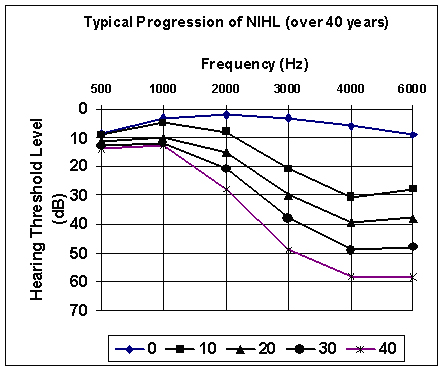
\includegraphics[width=0.48\textwidth]{images/nihl_graph.jpg}
  \end{center}
  \caption{NIHL: Noice Induce Hearing Loss}
\end{wrapfigure}
Our hearing can be impaired, either from natural causes or by accidents.


Causes can include:

\begin{itemize}
	\item Old age
	\item Heraditary causes
	\item Infections
	\item Acoustic trauma
\end{itemize}

Luckyly we are not reduced to use the old hearing horns or conversation tubes. We have DSP!
% subsection hearing_impairment (end)

% section dsp_in_hearing_aids (end)
\end{document}